\documentclass[11pt]{beamer}
\usetheme{Montpellier}
\usepackage[utf8]{inputenc}
\usepackage[portuguese]{babel}
\usepackage[T1]{fontenc}
\usepackage{amsmath}
\usepackage{amsfonts}
\usepackage{amssymb}
\usepackage{graphicx}
\usepackage{cases}
\usepackage{booktabs}
\usepackage{float}
\usepackage{tabularx}
\usepackage{caption}
\usepackage{scalefnt}

\newcommand\setItemnumber[1]{\setcounter{enumi}{\numexpr#1-1\relax}}


\author{Pedro Cunha\thanks{Mestrando - PPGE/UFPB} \and Rony Ramos\thanks{Mestrando - PPGE/UFPB} \and Valber Santos\thanks{Doutorando - PPGE/UFPB}}
\title{Uma avaliação da validade da Lei de Okun para o Brasil no período 1991-2019}
%\setbeamercovered{transparent} 
\setbeamertemplate{navigation symbols}{} 
\institute{Programa de Pós-Graduação em Economia Aplicada - UFPB} 
%\date{} 
\subject{Macroeconomia I - prof. Dr. Edilean Aragón} 
\begin{document}

\begin{frame}
\titlepage
\end{frame}

\begin{frame}
\tableofcontents
\end{frame}

\section{Introdução}

\begin{frame}{Objetivos do artigo}

\begin{enumerate}

\item Verificar o ajuste da Lei de Okun para movimentos de curto-prazo no desemprego, considerando dados para o Brasil desde 1991 até 2019;

\item Verificar a estabilidade da relação estimada ao longo do tempo.

\end{enumerate}

\end{frame}

\begin{frame}{Lei de Okun}

Assume-se que mudanças na demanda agregada fazem o produto flutuar ao redor do seu valor potencial. Essas mudanças no produto causam a contratação e demissão de trabalhadores pelas firmas, alterando o emprego; variações no emprego movem o desemprego no sentido oposto. Essas relações podem ser vistas no sistema de equações a seguir:
\begin{numcases}{}
E_t - E_t^*= \gamma \cdot (Y_t - Y_t^*) + \eta_t, \quad \gamma > 0 \\ 
U_t - U_t^* = \delta \cdot (E_t - E_t^*) + \mu_t, \quad \delta < 0 \\
U_t - U_t^* = \beta \cdot (Y_t - Y_t^*) + \epsilon_t, \quad \beta < 0 
\end{numcases}
onde $\beta = \delta \cdot \gamma$ e $\epsilon_t = \mu_t + \delta \cdot \eta_t$. Além disso, $E_t$ e $Y_t$ são o logaritmo do produto e do emprego, respectivamente, $U_t$ é a taxa de desemprego e $^*$ indica níveis de longo-prazo.
\end{frame}

\section{Como estimar a Lei de Okun?}

\begin{frame}{Estimação - "Níveis x Mudanças"}

\begin{enumerate}
    \item A primeira opção é estimar a equação $(3)$. O problema se encontra em estimar os termos não-observáveis $U_t^*$ e $Y_t^*$. Para contornar isso, foi utilizado o filtro \textit{Hodrick Prescott} (HP), que é bastante conhecido na literatura, muito embora tenha problemas de precisão;
    
    \item A segunda opção é estimar a versão "em mudanças" da Lei de Okun, dada pela equação a seguir:
    \begin{equation}
    \Delta U_t = \alpha + \beta \cdot \Delta Y_t + \omega_t
    \end{equation}
    onde $\Delta$ é a mudança em relação ao período anterior. Essa equação segue de $(3)$ se assumirmos que $U^*$ é constante e que $Y^*$ cresce a uma taxa constante ($\Delta Y^*$). Fazendo isso, obtemos a equação $(4)$ com $\alpha = -\beta \cdot \Delta Y^*$ e $\omega_t = \Delta \epsilon_t$.
\end{enumerate}

\end{frame}

\begin{frame}{Estimação - \textit{Seemingly Unrelated Regressions} (SUR)}

\begin{enumerate}
  \setItemnumber{3}
    \item Por fim, no interesse de estimar as relações econômicas derivadas do sistema composto pelas equações $(1), (2)$ e $(3)$ conjuntamente, foi utilizado o modelo de regressões aparentemente não-relacionadas, que será explicado mais a frente.
\end{enumerate}

\end{frame}

\section{Dados}

\begin{frame}{Fonte de dados}

\begin{table}[H]
\centering
\scriptsize
\caption*{Descrição das  variáveis}
\label{tab:dados}
\begin{tabularx}{\textwidth}{lcX} \\
Variável & Nome & Descrição \\ \midrule
$E_t$ & Emprego & $100 \times \ln(\text{tamanho total da força de trabalho})$ \\ \midrule
$U_t$ & Taxa de desemprego & $\%$ da força de trabalho desempregada que está ativamente procurando por um emprego \\ \midrule 
$Y_t$ & Produto & $100 \times \ln(\text{PIB em dólares correntes})$ \\ \bottomrule 
Fonte: & & The World Bank (2020).
\end{tabularx}
\end{table}

\end{frame}

\section{Metodologia}

\begin{frame}{Filtro Hodrick-Prescott}
\small 
A ideia básica por trás do filtro é a de \textbf{decomposição de uma série temporal}. Deixe $\{h_t\}_{t=1}^{T}$, denotar o logaritmo de uma variável de uma série temporal. Podemos decompor $h_t$ em um componente de tendência, $\tau_t$; um componente cíclico, $\pi_t$; e um componente de erro, $\epsilon_t$, de modo que 
\begin{equation}
h_t = \tau_t + \pi_t + \epsilon_t
\end{equation}
Considerando um parâmetro de ponderação, $\lambda$, escolhido de forma ótima, existe um componente de tendência $\tau_t^*$ que satisfaz o seguinte problema:
\begin{equation}
\underset{\tau_t^*}{\operatorname{min}} \left( \sum_{t=1}^T (h_t-\tau_t^*)^2 + \lambda \cdot \sum_{t=2}^{T-1} [(\tau_{t+1}^*-\tau_t^*) - (\tau_t^* - \tau_{t-1}^*)]^2 \right)
\end{equation}
O primeiro termo representa a soma dos quadrados dos desvios, $d_t = h_t - \tau_t^*$, que penaliza o componente cíclico. O segundo termo é uma ponderação da soma dos quadrados das segundas diferenças do componente de tendência. Esse termo penaliza variações na taxa de crescimento do componente de tendência.

\end{frame}

\begin{frame}{\textit{Seemingly Unrelated Regressions} (SUR)}

É uma generalização do modelo de regressão linear, sendo composto por várias equações de regressões, cada uma com suas respectivas variáveis dependentes e conjuntos potencialmente diferentes de variáveis explicativas.
\begin{numcases}{}
E_t - E_t^*= \gamma \cdot (Y_t - Y_t^*) + \eta_t, \quad \gamma > 0 \\ 
U_t - U_t^* = \delta \cdot (E_t - E_t^*) + \mu_t, \quad \delta < 0 \\
U_t - U_t^* = \beta \cdot (Y_t - Y_t^*) + \epsilon_t, \quad \beta < 0 
\end{numcases}
Cada equação do sistema acima pode ser estimada separadamente utilizando Mínimos Quadrados Ordinários, obtendo resultados que são consistentes. Entretanto, no caso em que os termos de erros das equações são correlacionados, tem-se um ganho de eficiência ao estimar as equações conjuntamente, fazendo uso, por exemplo, do método dos Mínimos Quadrados Generalizados Factíveis (MQGF).

\end{frame}

\begin{frame}{Quebra estrutural - teste de Chow e critério do menor \textit{Bayesian Information Criteria} (BIC)}

\begin{itemize}
    \item Para cada potencial ponto de mudança em um intervalo de tempo especificado, uma estatística F é calculada (estatística do teste de Chow). À partir disso, um modelo OLS é estimado para as observações de antes e depois do ponto de mudança e a soma dos quadrados dos resíduos é calculada (ESS). Um outro modelo é estimado para todas as observações, gerando uma soma de quadrados restritas (RSS). Se $n$ é o número de obervações e $k$ é o número de regressores no modelo, então:
    \begin{equation} \scriptsize
    F = \frac{RSS - ESS}{ESS \cdot (n - 2k)}
    \end{equation}
    \item A ideia do critério BIC é semelhante, porém em vez de comparar os valores da estatística de Chow com os críticos da distribuição F, é escolhido o número de quebras que gera o menor valor para o BIC.
\end{itemize}

\end{frame}

\section{Decomposições}

\begin{frame}{Decomposição da série temporal do desemprego}

\begin{figure}[H]
	\centering
	\label{fig:decomposição_desemprego}
	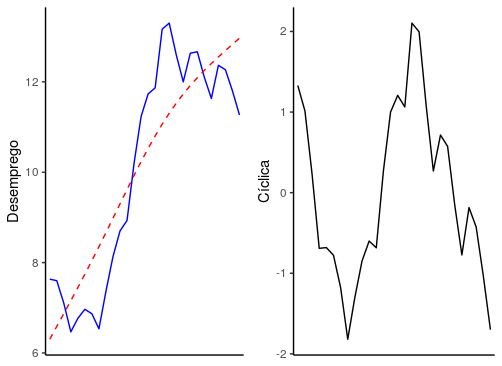
\includegraphics[height = 0.5\textheight, width=0.65\linewidth]{"Figuras/decomposição_desemprego.png"} \\
\caption*{Fonte: Elaboração própria à partir dos dados disponíveis em \textit{The World Bank}.}
\end{figure}

\end{frame}

\begin{frame}{Decomposição da série temporal do emprego}

\begin{figure}[H]
	\centering
	\label{fig:decomposição_emprego}
	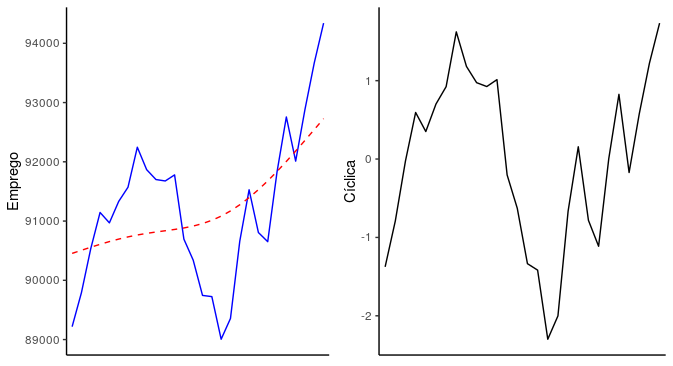
\includegraphics[height = 0.5\textheight, width=0.65\linewidth]{"Figuras/decomposição_emprego.png"} \\
\caption*{Fonte: Elaboração própria à partir dos dados disponíveis em \textit{The World Bank}.}
\end{figure}

\end{frame}

\begin{frame}{Decomposição da série temporal do PIB}

\begin{figure}[H]
	\centering
	\label{fig:decomposição_pib}
	\includegraphics[height = 0.5\textheight, width=0.65\linewidth]{"Figuras/decomposição_pib.png"} \\
\caption*{Fonte: Elaboração própria à partir dos dados disponíveis em \textit{The World Bank}.}
\end{figure}

\end{frame}

\section{Ball, Leigh e Loungani (2012)}

\begin{frame}{}

\centering Resultados: Okun's Law: Fit at 50?  - (BALL, LEIGH e LOUGANI, 2012)

\end{frame}

\begin{frame}{Resultados para os EUA}

\begin{itemize}
    \item A Lei de Okun se mostrou forte e estável (não houve quebra estrutural durante a grande recessão).
\end{itemize}

\begin{figure}[H]
	\centering
	\label{fig:tabela_1}
	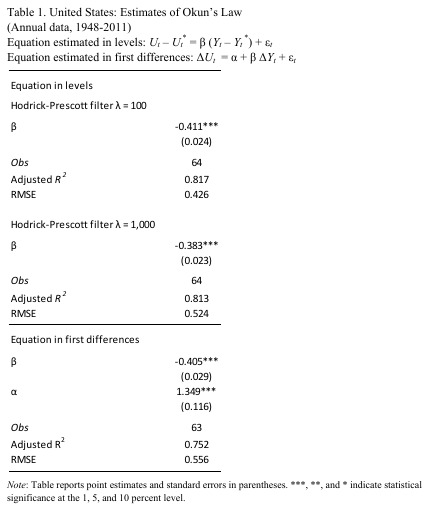
\includegraphics[height = 0.65\textheight, width=0.65\linewidth]{"Figuras/tabela_1.jpeg"} \\
\caption*{\small Fonte: (BALL, LEIGH e LOUGANI, 2012).}
\end{figure}

\end{frame}

\begin{frame}{Resultados para os EUA}

\begin{figure}[H]
	\centering
	\label{fig:tabela_3}
	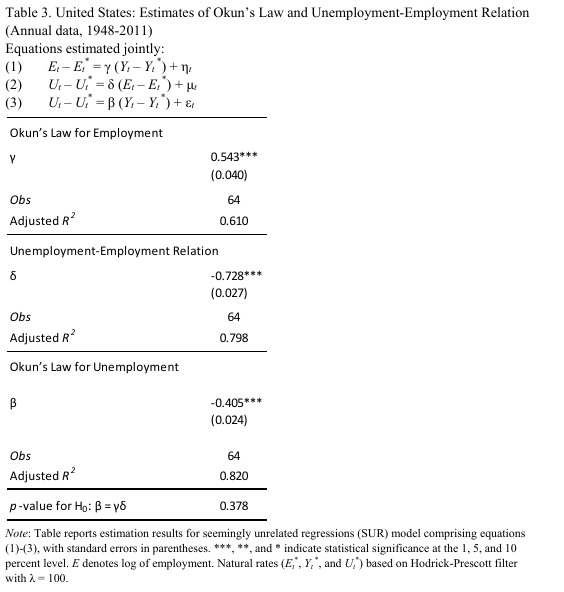
\includegraphics[height = 0.65\textheight, width=0.65\linewidth]{"Figuras/tabela_3.jpeg"} \\
\caption*{\small Fonte: (BALL, LEIGH e LOUGANI, 2012).}
\end{figure}

\end{frame}

\begin{frame}{Resultados para 20 economias avançadas}

\begin{itemize}
    \item Os dados se ajustam bem, porém, Austrália, Japão e Espanha apresentam resultados discrepantes.
\end{itemize}

\begin{figure}[H]
	\centering
	\label{fig:tabela_4}
	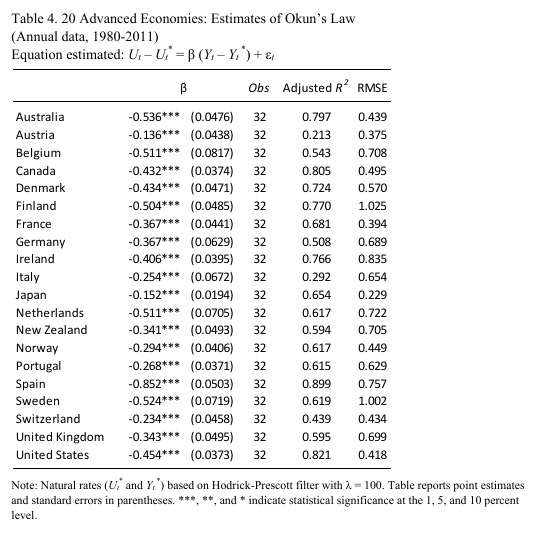
\includegraphics[height = 0.65\textheight, width=0.65\linewidth]{"Figuras/tabela_4.jpeg"} \\
\caption*{\small Fonte: (BALL, LEIGH e LOUGANI, 2012).}
\end{figure}

\end{frame}

\begin{frame}{Resultados para 20 economias avançadas}

\begin{itemize}
    \item Evidências de instabilidade para 7/20 países;
 
    \item Para 5 desses 7, o coeficiente da segunda metade é menor. O coeficiente médio da primeira metade é $-0,43$ e $-0,36$ na segunda metade, o que contraria o FMI (2010), que diz que o coeficiente aumentou ao longo do tempo em função de reformas legais, que reduziram os custos de demissão;
 \item Para os EUA, os coeficientes se mostraram estáveis. 
\end{itemize}  
 
\end{frame}

\begin{frame}{Resultados para 20 economias avançadas}

\begin{figure}[H]
	\centering
	\label{fig:tabela_5}
	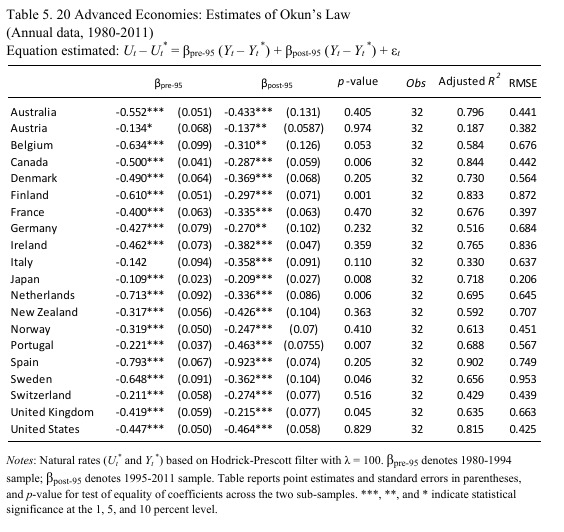
\includegraphics[height = 0.65\textheight, width=0.65\linewidth]{"Figuras/tabela_5.jpeg"} \\
\caption*{\small Fonte: (BALL, LEIGH e LOUGANI, 2012).}
\end{figure}

\end{frame}

\section{Resultados}

\begin{frame}{}

\centering Resultados: Uma avaliação da validade da Lei de Okun para o Brasil no período 1991-2019  - (CUNHA, RAMOS e SANTOS, 2020)

\end{frame}

\begin{frame}{Equação em níveis}

\begin{table}[H]
\centering
\caption*{Estimativas da Lei de Okun (dados anuais, 1991-2019)}
\label{tab:okun}
 \scalefont{0.65} 
\begin{tabular}{lc} \\ \multicolumn{2}{c}{$U_t - U_t^* = \beta \cdot (Y_t - Y_t^*) + \epsilon_t$} \\ \toprule
Filtro HP $\lambda = 100$ &  \\
$\beta$ & $-0,018^{**}$ \\
 & $(0,008)$ \\
Obs. & $29$ \\
$R^2$ ajustado & $0,122$ \\
RSE & $0,895$ (df = $28$) \\ \midrule
Filtro HP $\lambda = 1000$ &  \\
$\beta$ & $-0,033^{***}$ \\
 & $(0,008)$ \\
Obs. & $29$ \\
$R^2$ ajustado & $0,386$ \\
RSE & $1,133$ (df = $28$) \\ \midrule
\textit{Nota:} & $^*p < 0,1$; $^{**}p < 0,05$; $^{***}p < 0,01$ \\ \bottomrule
\end{tabular}
\end{table}

\end{frame}

\begin{frame}{Equação em primeiras diferenças}

\begin{table}[H]
\centering
\caption*{Estimativas da Lei de Okun (dados anuais, 1991-2019)}
\label{tab:okun_diferenças}
 \scalefont{0.75} 
\begin{tabular}{lc} \\ \multicolumn{2}{c}{$\Delta U_t = \alpha +  \beta \cdot \Delta Y_t + \epsilon_t$} \\ \toprule
$\beta$ & $-0,015$ \\
 & $(0,009)$ \\
$\alpha$ & $0,265$ \\
 & $(0,177)$ \\
Obs. & 28 \\
$R^2$ ajustado & $0,060$ \\
RSE & $0,918$ (df = $26$) \\ \midrule
\textit{Nota:} & $^*p < 0,1$; $^{**}p < 0,05$; $^{***}p < 0,01$ \\ \bottomrule
\end{tabular}
\end{table}

\end{frame}

\begin{frame}{Sistema de equações}

\begin{table}[H]
\centering
\caption*{\scriptsize Estimativas da Lei de Okun e da relação de Desemprego-Emprego(dados anuais, 1991-2016)}
\label{tab:sur}
\scalefont{0.5}
\begin{tabular}{@{}lc@{}}
\toprule
Lei de Okun para Emprego &  \\
$\gamma$ & $0,0138$ \\
 & $(0,0176)$ \\
Obs. & $26$ \\
$R^2$ ajustado & $0,0114$ \\
RSE & $6,2720$ (df = $25$) \\ \midrule
Relação Desemprego-Emprego &  \\
$\delta$ & $-0,1650^{**}$ \\
 & $(0,0570)$ \\
Obs. & $26$ \\
$R^2$ ajustado & $0,0955$ \\
RSE & $1,3986$ (df = $25$) \\ \midrule
Lei de Okun para Desemprego &  \\
$\beta$ & $-0,0114^{*}$ \\
 & $(0,0047)$ \\
Obs. & 26 \\
$R^2$ ajustado & $0,2496$ \\
RSE & $1,1604$ (df = $25$) \\ \midrule
p-valor para $H_0: \beta = \gamma \cdot \delta$ & $0,02464$ \\ \midrule
\textit{Nota:} & $^*p < 0,1$; $^{**}p < 0,05$; $^{***}p < 0,01$ \\ \bottomrule
\end{tabular}
\end{table}

\end{frame}

\subsection{Quebra estrutural}

\begin{frame}

\begin{figure}[H]
	\centering
	\caption*{Presença de quebra estrutural - Lei de Okun (1991-2019) - Critério do menor BIC - $\lambda = 1000$}
	\label{fig:quebra_estrutural}
	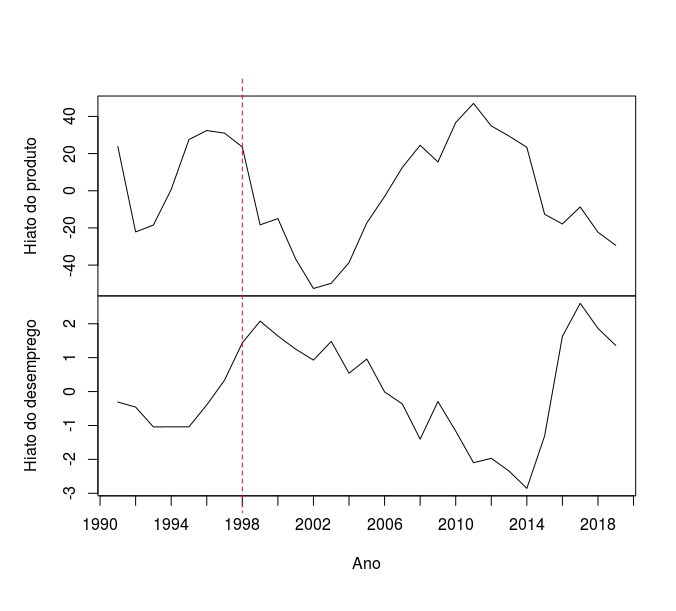
\includegraphics[width=0.70\linewidth]{"Figuras/quebra_estrutural.png"}
\end{figure}

\end{frame}


\begin{frame}

\begin{figure}[H]
	\centering
	\caption*{Presença de quebra estrutural - Lei de Okun (1991-2019) - Critério da estatística F - $\lambda = 1000$}
	\label{fig:quebra_estrutural_F}
	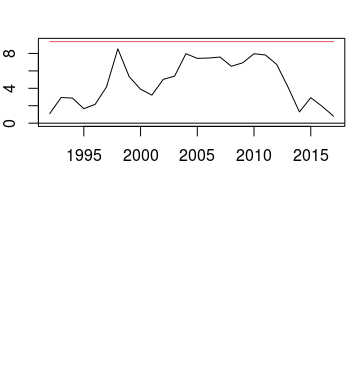
\includegraphics[width=0.75\linewidth]{"Figuras/quebra_estrutural_1000.png"}
\end{figure}

\end{frame}

\begin{frame}

\begin{table}[H]
\centering
\caption*{Lei de Okun (dados anuais, 1991-2019)} 
\label{tab:quebra_estrutural}
\scalefont{0.65}
\begin{tabular}{lc} \\ \multicolumn{2}{c}{$U_t - U_t^* = \beta \cdot (Y_t - Y_t^*) + \epsilon_t$
} \\ \toprule
Período $1991-1998$ &  \\
$\beta$ & $0,005$ \\
 & $(0,013)$ \\
Obs. & $8$ \\
$R^2$ ajustado & $-0,119$ \\
RSE & $0,907$ (df = $7$) \\ \midrule
Período $1999-2019$ &  \\
$\beta$ & $-0,043^{***}$ \\
 & $(0,008)$ \\
Obs. & 21 \\
$R^2$ ajustado & $0,587$ \\
RSE & $1,038$ (df = $20$) \\ \midrule
\textit{Nota}$^1$: & $^*p < 0,1$; $^{**}p < 0,05$; $^{***}p < 0,01$ \\ 
\textit{Nota}$^2$: & $U_t^*$ e $Y_t^*$ estimados utilizando o filtro HP com $\lambda = 1000$. \\
\end{tabular}
\end{table}

\end{frame}

\section{Considerações finais}

\begin{frame}{Considerações finais}

\begin{itemize}
    \item A Lei de Okun não se adequa tão bem aos dados brasileiros, em especial se considerado o sistema de equações completo e não apenas a relação desemprego-produto;
    \item Foi detectada a presença de uma quebra estrutural na equação estimada para a Lei de Okun considerando o critério de menor BIC, muito embora o teste de Chow aponte para a inexistência de quebra na equação estimada. A regressão realizada para o período \textbf{pós} 1998 apresentou o melhor ajuste à Lei de Okun, ao passo que para o período \textbf{pré} 1998 não foi obtido ajuste algum;
    \item Novos trabalhos devem buscar analisar o ajuste da Lei de Okun para outros países menos desenvolvidos, bem como outras metodologias de estimação, dado a notória discussão acerca da precisão do filtro HP.
\end{itemize}
    
\end{frame}

\section{}

\begin{frame}

\centering Obrigado!
    
\end{frame}

\end{document}